\section{Queueing theoretic model}

One of the main outcomes of this research is the creation of a queueing model
that consists of two waiting zones for two types of individuals.

\begin{figure}[h]
    \centering
    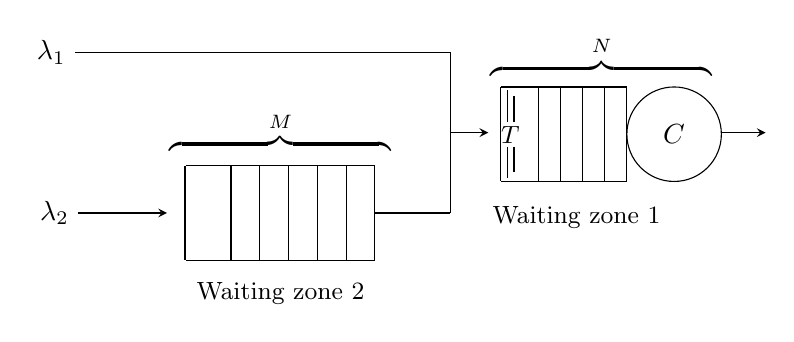
\begin{tikzpicture}[>=stealth, scale=0.8],
        % the rectangle of Queue 1
        \draw (0,0) -- ++(3cm,0) -- ++(0,-1.5cm) -- ++(-3cm,0);
        % The label above Queue 1 -> M
        \node[anchor=north] at (1.5cm, 1cm) {\(
            \overbrace{\qquad \qquad \qquad \qquad}^{M}
        \)};
        % The label below Queue 1 -> Waiting zone 2
        \node[anchor=north] at (1.5cm, -1.7cm) {\small{Waiting zone 2}};

        % the vertical lines in Queue 1
        \foreach \i in {1,...,5, 6.6}
        \draw (3cm-\i*13pt,0) -- +(0,-1.5cm);

        % % the circle in Queue 1
        % \draw (2.75,-0.75cm) circle [radius=0.75cm] node {\(0\)};

        % the rectangle in Queue 2
        \draw (5,1.25) -- ++(2cm,0) -- ++(0,-1.5cm) -- ++(-2cm,0);
        % the vertical lines in Queue 2
        \foreach \i in {1,...,4, 5.7}
        \draw (7cm-\i*10pt,1.25) -- +(0,-1.5cm);
        % The two vertical lines at the start of Queue 2
        \draw (7cm-54pt,1.2) -- +(0,-0.5cm);
        \draw (7cm-54pt,0.3) -- +(0,-0.5cm);
        \draw (7cm-51pt,1.1) -- +(0,-0.4cm);
        \draw (7cm-51pt,0.3) -- +(0,-0.4cm);

        % The label between the lines for T
        \node[anchor=north] at (5.15, 0.77 cm) {\small{\( T \)}};

        % The label above Queue 2 -> N
        \node[anchor=north] at (6.6cm, 2.2cm) {\(
            \overbrace{\qquad \qquad \qquad \qquad}^{N}
        \)};
        % The label below Queue 2 -> Waiting zone 1
        \node[anchor=north] at (6.2cm, -0.5cm) {\small{Waiting zone 1}};

        % the circle in Queue 2
        \draw (7.75,0.5) circle [radius=0.75cm] node {\(C\)};

        % Arrow line from Queue 2 outside
        \draw[->] (8.5,0.525) -- +(20pt,0);

        % Line from lambda_2 to Queue 1
        \draw[<-] (-0.3,-0.75) -- +(-40pt,0) node[left] {\( \lambda_2 \)};
        % First line (horizontal) after Queue 1
        \draw[-] (3,-0.75) -- +(34pt,0);
        % Second line (vertical) after Queue 1
        \draw (4.2, 0.525) -- (4.2, -0.75);

        % First line (horizontal) from lambda_1
        \draw (4.2, 1.8) -- +(-169.5pt,0) node[left] {\( \lambda_1 \)};
        % Second line (vertical) from lambda_1
        \draw (4.2, 1.8) -- (4.2, 0.525);
        % Arrow line to Queue 2
        \draw[->] (4.2, 0.525) -- (4.8, 0.525);
    \end{tikzpicture}
    \caption{A diagrammatic representation of the queueing network.
    The threshold \(T\) only applies to type 2 individuals.
    If the number of individuals in waiting zone 1 is greater than or equal to
    \(T\), only individuals of type 1 are accepted (at a rate \(\lambda_1\))
    and individuals of type 2 (arriving at a rate \(\lambda_2\)) are blocked in
    waiting zone 2.}
    \label{fig:diagram_of_queueing_system}
\end{figure}


The model consists of two types of individuals; type 1 and type 2.
Type 1 individuals arrive instantly at waiting zone 1 and wait to receive their
service.
Type 2 individuals arrive at waiting zone 2 and wait there until they are
allowed to move to waiting zone 1.
They are allowed to proceed only when the number of
individuals in waiting zone 1 \textbf{and} in service is less than a
pre-determined threshold \(T\).
When the number of individuals is equal to or exceeds this threshold, all
type 2 individuals that arrive will stay \textit{blocked} in waiting zone 2 
until the number of people in waiting zone 1 falls below \(T\).
This is shown diagrammatically in Figure \ref{fig:diagram_of_queueing_system}.
The parameters of the described queueing model are:

\begin{itemize}
    \item \(\lambda_i\): The arrival rate of type \(i\) individuals where
    \(i\in\{1, 2\}\)
    \item \(\mu\): The service rate for individuals receiving service after
    waiting zone 1
    \item \(C\): The number of servers
    \item \(T\): The threshold at which individuals of the second type are
    blocked
\end{itemize}

\subsection{Markov chain}

Under the assumption that all rates (arrival and service) are Markovian the
queueing system corresponds to a Markov chain~\cite{kemeny1976markov}.
The states of the Markov chain are denoted by \((u,v)\) where:

\begin{itemize}
    \item \(u\) is the number of individuals blocked
    \item \(v\) is the number of individuals either in waiting zone 1 or in the
    service centre
\end{itemize}

We denote the state space of the Markov chain as  \(S=S(T)\) which can be
written as the disjoint union (\ref{eq:definition_of_S_as_disjoint_union}).

\begin{align}
    S(T) =& S_1(T) \cup S_2(T) \text{ where:} \nonumber \\
    S_1(T) =& \left\{(0, v)\in\mathbb{N}_0^2 \; | \; v < T \right\}
    \label{eq:definition_of_S_as_disjoint_union} \\
    S_2(T) =& \{(u, v)\in\mathbb{N}_0^2 \; | \; v \geq T \} \nonumber
\end{align}




\subsubsection{Generator matrix}

The generator matrix \(Q\) of the Markov chain consists of the
rates between the numerous states of the model.
Every entry \( Q_{ij} = Q_{(u_i, v_i),(u_j, v_j)} \) represents the rate from
state \( i = (u_i, v_i) \) to state \( j = (u_j , v_j) \) for all
\( (u_i, v_i), (u_j, v_j) \in S \).
The entries of \(Q\) can be calculated using the state-mapping function
described in (\ref{eq:markov_transition_rate}):

\begin{equation} \label{eq:markov_transition_rate}
    Q_{ij} =
    \begin{cases}
        \Lambda, & \textbf{if } (u_i, v_i) - (u_j, v_j) = (0,-1) \textbf{ and }
        v_i < \text{t} \\
        \lambda_1, & \textbf{if } (u_i, v_i) - (u_j, v_j) = (0,-1)
        \textbf{ and } v_i \geq \text{t} \\
        \lambda_2, & \textbf{if } (u_i, v_i) - (u_j, v_j) = (-1,0) \\
        v_i \mu, & \textbf{if } (u_i, v_i) - (u_j, v_j) = (0,1) \textbf{ and }
        v_i \leq C \textbf{ or} \\ & \hspace{0.37cm}(u_i, v_i) - (u_j, v_j) =
        (1,0) \textbf{ and } v_i = T \leq C \\
        C \mu, & \textbf{if } (u_i, v_i) - (u_j, v_j) = (0,1) \textbf{ and }
        v_i > C
        \textbf{ or} \\ & \hspace{0.37cm}(u_i, v_i) - (u_j, v_j) = (1,0)
        \textbf{ and } v_i = T > C\\
        -\sum_{j=1}^{|Q|}{Q_{ij}} & \textbf{if } i = j \\
        0, & \textbf{otherwise}
    \end{cases}
\end{equation}

Note that \(\Lambda\) here denotes the overall arrival rate in the model by both
types of individuals (i.e. \(\Lambda = \lambda_1 + \lambda_2\)).
A visualisation of how the transition rates relate to the states of the model
can be seen in the general Markov chain model shown in Figure
\ref{fig:general_markov_model}.

\begin{figure}[H]
    \centering
    \scalebox{.8}
    {
        \begin{tikzpicture}[-, node distance = 0.9cm, auto, every node/.style={scale=0.7}]

            % Markov chain variables
            \tikzmath{
                let \initdist = 0.5cm;
                let \altdist = 1.2cm;
                let \minsz = 1.6cm;
            }

            % S_1 and S_2 rectangles
            \tikzmath{
                let \leftOne = -0.8;
                let \rightOne = 2.7;
                let \upOne = 0.8;
                let \downOne = -2.7;
                let \leftTwo = 2.8;
                let \rightTwo = 13;
                let \upTwo = -2.95;
                let \downTwo = -16.4;
            }

            % General case variables
            \tikzmath{
                let \GCsmallx = 8.3;
                let \GCsmally = -9.5;
                let \GCbigx = 4.1;
                let \GCbigy = -11.8;
            }

            % Rectangle for S1
            \draw[ultra thin, dashed] (\leftOne, \downOne) -- (\leftOne, \upOne);
            \draw[ultra thin, dashed] (\leftOne, \upOne) -- (\rightOne, \upOne);
            \draw[ultra thin, dashed] (\rightOne, \upOne) -- node 
            {\Huge{\( \quad S_1 \)}}(\rightOne, \downOne);
            \draw[ultra thin, dashed] (\rightOne, \downOne) -- (\leftOne, \downOne);

            % Rectangle for S2
            \draw[ultra thin, dashed] (\leftTwo, \downTwo) -- node 
            {\Huge{\( S_2 \quad \)}}(\leftTwo, \upTwo);
            \draw[ultra thin, dashed] (\leftTwo, \upTwo) -- (\rightTwo, \upTwo);
            \draw[ultra thin, dashed] (\rightTwo, \upTwo) -- (\rightTwo, \downTwo);
            \draw[ultra thin, dashed] (\rightTwo, \downTwo) -- (\leftTwo, \downTwo);

            % Small square of general case
            \draw [thick] (\GCsmallx, \GCsmally) -- node {} 
            (\GCsmallx + 0.4, \GCsmally);
            \draw [thick] (\GCsmallx + 0.4, \GCsmally) -- node {} 
            (\GCsmallx + 0.4, \GCsmally - 0.4);
            \draw [thick] (\GCsmallx + 0.4, \GCsmally - 0.4) -- node {} 
            (\GCsmallx, \GCsmally - 0.4);
            \draw [thick] (\GCsmallx, \GCsmally - 0.4) -- node {} 
            (\GCsmallx, \GCsmally);


            % Dashed lines to from small square to big one 
            \draw [ultra thin] (\GCsmallx, \GCsmally) -- node {} 
            (\GCbigx, \GCbigy);
            \draw [ultra thin] (\GCsmallx + 0.4, \GCsmally) -- node {} 
            (\GCbigx + 4, \GCbigy);
            \draw [ultra thin] (\GCsmallx, \GCsmally - 0.4) -- node {} (7, \GCbigy);
            \draw [ultra thin] (\GCsmallx + 0.4, \GCsmally - 0.4) -- node {} 
            (\GCbigx + 4, \GCbigy - 4);
            
            % Big Square of general case
            \draw [ultra thick] (\GCbigx, \GCbigy) -- node {} (\GCbigx + 4, \GCbigy);
            \draw [ultra thick] (\GCbigx + 4, \GCbigy) -- node {} 
            (\GCbigx + 4, \GCbigy - 4);
            \draw [ultra thick] (\GCbigx + 4, \GCbigy - 4) -- node {General Case} 
            (\GCbigx, \GCbigy - 4);
            \draw [ultra thick] (\GCbigx, \GCbigy - 4) -- node {} (\GCbigx, \GCbigy);

            % First Line
            \node[state, minimum size=1.5cm] (zero) {(0,0)};
            \node[state, node distance = \initdist, minimum size=\minsz, below right=of zero] 
            (one) {(0,1)};
            \node[draw=none, node distance = \initdist, minimum size=\minsz, below right=of one] 
            (two) {\textbf{\( \ddots \)}};
            \node[state, node distance = \initdist, minimum size=\minsz, below right=of two] 
            (three) {(0,T)};
            \node[state, node distance = \altdist, minimum size=\minsz, right=of three] 
            (four) {(0,T+1)};
            \node[draw=none, node distance = \altdist, minimum size=\minsz, right=of four] 
            (five) {\textbf{\dots}};
            \node[state, minimum size=\minsz, right=of five] (six) {(0,C)};
            \node[draw=none, minimum size=\minsz, right=of six] (seven) {\textbf{\dots}};

            % Second Line
            \node[state, minimum size=\minsz, below=of three] (three_one) {(1,T)};
            \node[state, minimum size=\minsz, below=of four] (four_one) {(1,T+1)};
            \node[draw=none, minimum size=\minsz, below=of five] (five_one) {\textbf{\dots}};
            \node[state, minimum size=\minsz, right=of five_one] (six_one) {(1,C)};
            \node[draw=none, minimum size=\minsz, right=of six_one] (seven_one) {\textbf{\dots}};
            
            % Third Line
            \node[state, minimum size=\minsz, below=of three_one] (three_two) {(2,T)};
            \node[state, minimum size=\minsz, below=of four_one] (four_two) {(2,T+1)};
            \node[draw=none, minimum size=\minsz, below=of five_one] (five_two) 
            {\textbf{\dots}};
            \node[state, minimum size=\minsz, right=of five_two] (six_two) {(2,C)};
            \node[draw=none, minimum size=\minsz, right=of six_two] (seven_two) 
            {\textbf{\dots}};

            % Fourth line
            \node[draw=none, node distance = \altdist, minimum size=\minsz, below=of three_two] 
            (three_three) {\textbf{\vdots}};
            \node[draw=none, node distance = \altdist, minimum size=\minsz, below=of four_two] 
            (four_three) {\textbf{\vdots}};
            \node[draw=none, node distance = 2cm, minimum size=\minsz, below=of five_two] 
            (five_three) {};
            \node[draw=none, node distance = \altdist, minimum size=\minsz, below=of six_two] 
            (six_three) {\textbf{\vdots}};

            % Fifth line
            \node[draw=none, node distance = 0.3cm, minimum size=\minsz, below=of four_three] 
            (general_case_up) {};
            \node[state, node distance = \altdist, minimum size=\minsz, below=of general_case_up] 
            (general_case_mid) {\( (u_i, v_i) \)};

            \node[draw=none, node distance = \altdist, minimum size=\minsz, below=of general_case_mid] 
            (general_case_down) {};
            \node[draw=none, node distance = \altdist, minimum size=\minsz, left=of general_case_mid] 
            (general_case_left) {};
            \node[draw=none, node distance = \altdist, minimum size=\minsz, right=of general_case_mid] 
            (general_case_right) {};

            \draw[every loop]
                % First Horizontal Edges
                (zero) edge[bend left] node {\( \Lambda \)} (one)
                (one) edge[bend left] node {\( \mu \)} (zero)
                (one) edge[bend left] node {\( \Lambda \)} (two)
                (two) edge[bend left] node {\( 2 \mu \)} (one)
                (two) edge[bend left] node {\( \Lambda \)} (three)
                (three) edge[bend left] node {\( T \mu \)} (two)
                (three) edge[bend left] node {\( \lambda_1 \)} (four)
                (four) edge[bend left] node {\( (T+1) \mu \)} (three)
                (four) edge[bend left] node {\( \lambda_1 \)} (five)
                (five) edge[bend left] node {\( (T+2) \mu \)} (four)
                (five) edge[bend left] node {\( \lambda_1 \)} (six)
                (six) edge[bend left] node {\( C\mu \)} (five)
                (six) edge[bend left] node {\( \lambda_1 \)} (seven)
                (seven) edge[bend left] node {\( C\mu \)} (six)

                % Second Horizontal Edges
                (three_one) edge[bend left] node {\( \lambda_1 \)} (four_one)
                (four_one) edge[bend left] node {\( (T+1) \mu \)} (three_one)
                (four_one) edge[bend left] node {\( \lambda_1 \)} (five_one)
                (five_one) edge[bend left] node {\( (T+2) \mu \)} (four_one)
                (five_one) edge[bend left] node {\( \lambda_1 \)} (six_one)
                (six_one) edge[bend left] node {\( C\mu \)} (five_one)
                (six_one) edge[bend left] node {\( \lambda_1 \)} (seven_one)
                (seven_one) edge[bend left] node {\( C\mu \)} (six_one)

                % Third Horizontal Edges
                (three_two) edge[bend left] node {\( \lambda_1 \)} (four_two)
                (four_two) edge[bend left] node [below] {\( (T+1) \mu \)} (three_two)
                (four_two) edge[bend left] node {\( \lambda_1 \)} (five_two)
                (five_two) edge[bend left] node {\( (T+2) \mu \)} (four_two)
                (five_two) edge[bend left] node {\( \lambda_1 \)} (six_two)
                (six_two) edge[bend left] node {\( C\mu \)} (five_two)
                (six_two) edge[bend left] node {\( \lambda_1 \)} (seven_two)
                (seven_two) edge[bend left] node {\( C\mu \)} (six_two)

                % First Vertical Edges
                (three) edge[bend left] node {\( \lambda_2 \)} (three_one)
                (three_one) edge[bend left] node {\( T \mu \)} (three)
                (three_one) edge[bend left] node {\( \lambda_2 \)} (three_two)
                (three_two) edge[bend left] node {\( T\mu \)} (three_one)
                (three_two) edge[bend left] node {\( \lambda_2 \)} (three_three)
                (three_three) edge[bend left] node {\( T\mu \)} (three_two)

                % Second Vertical Edges
                (four) edge node {\( \lambda_2 \)} (four_one)
                (four_one) edge node {\( \lambda_2 \)} (four_two)
                (four_two) edge node {\( \lambda_2 \)} (four_three)

                % Fourth Vertical Edges
                (six) edge node {\( \lambda_2 \)} (six_one)
                (six_one) edge node {\( \lambda_2 \)} (six_two)
                (six_two) edge node {\( \lambda_2 \)} (six_three)

                % General Case
                (general_case_left) edge[bend left] node {\( \lambda_1 \)} (general_case_mid)
                (general_case_mid) edge[bend left] node {\( v_i \mu \)} (general_case_left)
                (general_case_right) edge[bend left] node {\( (v_i +1) \mu \)} (general_case_mid)
                (general_case_mid) edge[bend left] node {\( \lambda_1 \)} (general_case_right)
                % (five_three) edge node {\( \lambda_2 \)} (general_case_mid)
                (general_case_up) edge node {\( \lambda_2 \)} (general_case_mid)
                (general_case_mid) edge node {\( \lambda_2 \)} (general_case_down)
                ;
        \end{tikzpicture}
    }
    \caption{General case of the Markov chain model} 
    \label{fig:general_markov_model}
\end{figure}


In order to consider this model numerically an adjustment needs to be made.
The problem defined above assumes no upper boundary to the number of individuals
that can wait for service or for the ones that are blocked in the buffer centre.
Therefore, a different state space \( \tilde S \) is constructed where
\( \tilde S \subseteq S \) and there is a maximum allowed number of individuals
\(N\) that can be in the system and a maximum allowed number of individuals
\(M\) that can be blocked in the buffer centre:

\begin{equation}
    \tilde S = \left\{ (u, v) \in S\;| u \leq M, v\leq N \right\}
\end{equation}



\subsubsection{Steady state}
The generator matrix \( Q \) defined in (\ref{eq:markov_transition_rate}) can
be used to get the probability vector \( \pi \).
The vector \( \pi \) is commonly used to study stochastic systems and it's main
purpose is to keep track of the probability of being at any given state of
the system.
\(\pi_i\) is the steady state probability of being in state \((u_i, v_i) \in
\tilde S\) which is the \(i^{\text{th}}\) state of \(\tilde S\) for some ordering of
\(\tilde S\).
The term \textit{steady state} refers to the instance of the vector \( \pi \)
where the probabilities of being at any state become stable over time.
Thus, by considering the steady state vector \( \pi \) the relationship between
it and \( Q \) is given by:

\[
    \frac{d\pi}{dt} = \pi Q = 0
\]

\subsubsection{Graph theoretic approach to steady state}


\subsection{Performance measures}
Using vector \(\pi\) there are numerous performance measures of the model that
can be calculated.
The following equations utilise \(\pi\) to get performance measures on the
average number of people at certain sets of state:

\begin{itemize}
    \item Average number of people in the system:
        \[L = \sum_{i=1}^{|\pi|} \pi_i (u_i + v_i)\]
    \item Average number of people in the service centre:
        \[L_H = \sum_{i=1}^{|\pi|} \pi_i v_i\]
    \item Average number of people in waiting zone 2:
        \[L_A = \sum_{i=1}^{|\pi|} \pi_i u_i\]
\end{itemize}

Consequently, there are some additional performance measures of interest that
are not as straightforward to calculate.
Such performance measures are the mean waiting time in the system (for both
type 1 and type 2 individuals), the mean time blocked in waiting zone 2 (only
valid for type 2 individuals) and the proportion of individuals that wait in
waiting zone 1 within a predefined time target (for both types).

\subsubsection{Waiting time}
\subsubsection{Blocking time}
\subsubsection{Proportion of individuals within target}

